\documentclass[a4paper, 11pt]{article}
\usepackage{comment} % enables the use of multi-line comments (\ifx \fi) 
\usepackage{fullpage} % changes the margin
\usepackage[a4paper, total={7in, 10in}]{geometry}
\usepackage{amsmath,mathtools,mathdots}
\usepackage{amssymb,amsthm}  % assumes amsmath package installed
\usepackage{float}
\usepackage{xcolor}
\usepackage{mdframed}
\usepackage[shortlabels]{enumitem}
\usepackage{indentfirst}
\usepackage{hyperref}
\hypersetup{
	colorlinks=true,
	linkcolor=doc!80,
	citecolor=myr,
	filecolor=myr,      
	urlcolor=doc!80,
	pdftitle={Assignment}, %%%%%%%%%%%%%%%%   WRITE ASSIGNMENT PDF NAME  %%%%%%%%%%%%%%%%%%%%
}
\usepackage[most,many,breakable]{tcolorbox}
\usepackage{tikz}
\usepackage{caption}
\usepackage{mathpazo}
% Use the libertine package for the Libertine font
\usepackage{libertine}
\usepackage[libertine]{newtxmath}
\usepackage{libertine}
\usepackage{physics}
\usepackage[ruled,vlined,linesnumbered]{algorithm2e}
\usepackage{mathrsfs}
\usepackage{tikz-cd}
\usepackage{float}

\definecolor{mytheorembg}{HTML}{F2F2F9}
\definecolor{mytheoremfr}{HTML}{00007B}
\definecolor{doc}{RGB}{0,60,110}
\definecolor{myg}{RGB}{56, 140, 70}
\definecolor{myb}{RGB}{45, 111, 177}
\definecolor{myr}{RGB}{199, 68, 64}

\usetikzlibrary{decorations.pathreplacing,angles,quotes,patterns}
\definecolor{mytheorembg}{HTML}{F2F2F9}
\definecolor{mytheoremfr}{HTML}{00007B}
\definecolor{doc}{RGB}{0,60,110}
\definecolor{myg}{RGB}{56, 140, 70}
\definecolor{myb}{RGB}{45, 111, 177}
\definecolor{myr}{RGB}{199, 68, 64}

\tcbuselibrary{theorems,skins,hooks}
\newtcbtheorem{problem}{Problem}
{%
	enhanced,
	breakable,
	colback = mytheorembg,
	frame hidden,
	boxrule = 0sp,
	borderline west = {2pt}{0pt}{mytheoremfr},
	arc=5pt,
	detach title,
	before upper = \tcbtitle\par\smallskip,
	coltitle = mytheoremfr,
	fonttitle = \bfseries\sffamily,
	description font = \mdseries,
	separator sign none,
	segmentation style={solid, mytheoremfr},
}
{p}

\newtheorem{lemma}{Lemma}
\renewenvironment{proof}{\noindent{\it \textbf{Proof:}}\hspace*{1em}}{\qed\bigskip\\}
% To give references for any problem use like this
% suppose the problem number is p3 then 2 options either 
% \hyperref[p:p3]{<text you want to use to hyperlink> \ref{p:p3}}
%                  or directly 
%                   \ref{p:p3}



\input{../../letterfonts}

\input{../../macros}

\setlength{\parindent}{0pt}

%%%%%%%%%%%%%%%%%%%%%%%%%%%%%%%%%%%%%%%%%%%%%%%%%%%%%%%%%%%%%%%%%%%%%%%%%%%%%%%%%%%%%%%%%%%%%%%%%%%%%%%%%%%%%%%%%%%%%%%%%%%%%%%%%%%%%%%%

\begin{document}
	
	%%%%%%%%%%%%%%%%%%%%%%%%%%%%%%%%%%%%%%%%%%%%%%%%%%%%%%%%%%%%%%%%%%%%%%%%%%%%%%%%%%%%%%%%%%%%%%%%%%%%%%%%%%%%%%%%%%%%%%%%%%%%%%%%%%%%%%%%
	
	\textsf{\noindent \large\textbf{Soham Chatterjee} \hfill \textbf{Assignment - 2}\\
		Email: \href{soham.chatterjee@tifr.res.in}{soham.chatterjee@tifr.res.in} \hfill Dept: STCS\\
		\normalsize Course: Probability Theory \hfill Date: \today}
	
%%%%%%%%%%%%%%%%%%%%%%%%%%%%%%%%%%%%%%%%%%%%%%%%%%%%%%%%%%%%%%%%%%%%%%%%%%%%%%%%%%%%%%%%%%%%%%%%%%%%%%%%%%%%%%%%%%%%%%%%%%%%%%%%%%%%%%%%
% Problem 1
%%%%%%%%%%%%%%%%%%%%%%%%%%%%%%%%%%%%%%%%%%%%%%%%%%%%%%%%%%%%%%%%%%%%%%%%%%%%%%%%%%%%%%%%%%%%%%%%%%%%%%%%%%%%%%%%%%%%%%%%%%%%%%%%%%%%%%%%
	
\begin{problem}{%problem statement
		[H] Problem 1.3: Ordering of three random variables
	}{p1% problem reference text
}
Suppose $X,Y$ and $U$ are mutually independent, such that $X$ and $Y$ are each exponentially distributed with some common parameter $\lm>0$ and $U$ is uniformly distributed on the interval $[0,1]$. Express $\bbP\{X<U<Y\}$ in terms of $\lm$. Simplify your answer.
\end{problem}
\solve{
$X$ and $Y$ are exponentially distributed with some common parameter $\lm>0$. Hence $F_X(x)=1- e^{-\lm x}$ and $F_Y(y)=1- e^{-\lm y}$ for some $x,y\geq 0$.and $U$ is uniform on $[0,1]$. So \begin{align*}
	\bbP[X<U<Y] & =\int_0^1\bbP[X< u, Y>u]du\\
	& = \int_0^1\bbP[X<u]\cdot \bbP[Y>u]du\\
	& = \int_0^1F_X(u)(1-F_Y(u))du\\
	& = \int_0^1 \lt(1-e^{-\lm u}\rt)\lt(1-\lt(1-e^{\lm u}\rt)\rt)du\\
	& = \int_0^1\lt(1-e^{-\lm u}\rt)e^{-\lm u}du\\
	& = \int_0^1 \lt[e^{-\lm u}-e^{-2\lm u}\rt]du\\
	& = \lt[\frac{e^{-\lm u}}{-\lm}-\frac{e^{-2\lm u}}{-2\lm}\rt]_0^1\\
	& = \lt[\frac{e^{-2\lm }}{2\lm}-\frac{e^{-\lm }}{\lm}\rt]-\lt[\frac{1}{2\lm}-\frac{1}{\lm}\rt] = \frac{\lt(e^{-\lm}\rt)^2-2e^{-\lm}+1}{2\lm}= \frac{\lt(e^{-\lm}-1\rt)^2}{2\lm}
\end{align*}
}
%%%%%%%%%%%%%%%%%%%%%%%%%%%%%%%%%%%%%%%%%%%%%%%%%%%%%%%%%%%%%%%%%%%%%%%%%%%%%%%%%%%%%%%%%%%%%%%%%%%%%%%%%%%%%%%%%%%%%%%%%%%%%%%%%%%%%%%%
% Problem 2
%%%%%%%%%%%%%%%%%%%%%%%%%%%%%%%%%%%%%%%%%%%%%%%%%%%%%%%%%%%%%%%%%%%%%%%%%%%%%%%%%%%%%%%%%%%%%%%%%%%%%%%%%%%%%%%%%%%%%%%%%%%%%%%%%%%%%%%%

\begin{problem}{%problem statement
		[H] Problem 1.5: Congestion at output ports
	}{p2% problem reference text
	}
Consider a packet switch with some number
of input ports and eight output ports. Suppose four packets simultaneously arrive
on different input ports, and each is routed toward an output port. Assume the
choices of output ports are mutually independent, and for each packet, each
output port has equal probability.\begin{enumerate}[label=(\alph*)]
	\item Specify a probability space $(\Om,\mcF,\bbP)$ to describe this situation.
	\item Let $X_i$ denote the number of packets routed to output port $i$ for $1\leq i\leq 8$. Describe the joint pmf of $X_1,\dots,X_8$.
	\item Find $\cov(X_1,X_2)$
	\item Find $\bbP[X_i\leq 1 \text{ for all $i$}]$
	\item Find $\bbP[X_i\leq 2 \text{ for all $i$}]$
\end{enumerate}
\end{problem}
\solve{
}

\newpage
%%%%%%%%%%%%%%%%%%%%%%%%%%%%%%%%%%%%%%%%%%%%%%%%%%%%%%%%%%%%%%%%%%%%%%%%%%%%%%%%%%%%%%%%%%%%%%%%%%%%%%%%%%%%%%%%%%%%%%%%%%%%%%%%%%%%%%%%
% Problem 3
%%%%%%%%%%%%%%%%%%%%%%%%%%%%%%%%%%%%%%%%%%%%%%%%%%%%%%%%%%%%%%%%%%%%%%%%%%%%%%%%%%%%%%%%%%%%%%%%%%%%%%%%%%%%%%%%%%%%%%%%%%%%%%%%%%%%%%%%

\begin{problem}{%problem statement
		[H] Problem 1.13: A CDF of mixed type
	}{p3% problem reference text
	}
Let $X$ have the CDF shown.

\begin{center}
	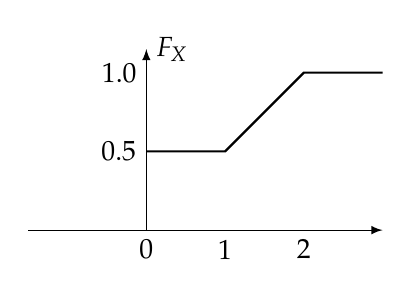
\begin{tikzpicture}
		\draw[-latex] (-1.5,0) -- (1,0) node[below] {$1$} -- (2,0) node[below]{$2$} -- (3,0);
		\draw[-latex] (0,0) node[below] {$0$} -- (0,2.3) node[above, right]{$F_X$};
		\draw[thick] (0,1) node[left] {$0.5$} -- (1,1) -- (2,2) -- (3,2); 
		\draw (0,2) node[left] {1.0};
	\end{tikzpicture}
\end{center}
\begin{enumerate}[label=(\alph*)]
	\item Find $\bbP[X\leq 0.8]$
	\item Find $\bbE[X]$
	\item Find $\Var [X]$
\end{enumerate}
\end{problem}
\solve{
\begin{enumerate}[label=(\alph*)]
	\item $\bbP[X\leq 0.8]=\bbF_X[0.8]=0.5$ since the value of $F_X$ increases when $X\geq 1$. 
	\item $F_X(x)=\begin{cases}
		0&\text{when $x\leq 0$}\\
		0.5 & \text{when} 0\leq x\leq 1\\
		0.5+\frac{x-1}2 & \text{when } 1\leq x\leq 2\\
		1& \text{when }x\geq 2
	\end{cases}$ 

Hence \begin{align*}
	\bbE[X]& =\int_0^{\infty}[1-F_X(x)]dx=\int_0^1[1-0.5]dx+\int_1^2\lt[1-0.5-\frac{x-1}2\rt]dx+\int_2^{\infty}[1-1]dx\\
	& =\int_0^10.5dx+\int_1^2\lt[0.5-\frac{x-1}2\rt]dx\\
	& = 0.5+\lt[0.5x-\frac{(x-1)^2}{4}\rt]^2_1= 1-\frac14=\frac34
\end{align*}
	\item Take $Y=X^2$ and the distribution function for $Y$ is $F_Y$. Now for any $y\geq 0$ $$F_Y(y)=\bbP[Y^2\leq y]=\bbP[X^2\leq y]=\bbP[X\leq \sqrt{y}]=F_X(\sqrt{y})$$
	Therefore $$F_Y(y)=\begin{cases}
		0&\text{when $x\leq 0$}\\
		0.5 & \text{when} 0\leq x\leq 1\\
		0.5+\frac{\sqrt{y}-1}2 & \text{when } 1\leq y\leq 4\\
		1& \text{when }y\geq 4
	\end{cases}$$Hence \begin{align*}
	\bbE[X^2] &  =\int_0^{\infty}[1-F_Y(y)]dy=\int_0^1[1-0.5]dy+\int_1^4\lt[1-0.5-\frac{\sqrt{y}-1}2\rt]dy+\int_4^{\infty}[1-1]dy\\
	& = \int_0^10.5dy+\int_1^4\lt[0.5-\frac{\sqrt{y}-1}{2}\rt]dy\\
	& = 0.5+\lt[ 0.5y-\frac{\frac23y^{\frac32}-y}{2} \rt]_1^4=0.5+3\cdot 0.5-\lt[ \frac{\frac234^{\frac32}-4}{2} - \frac{\frac231^{\frac32}-1}{2}\rt] =2 -\frac56=\frac{7}6
\end{align*}
So $\Var[X]=\bbE[X^2]-\bbE[X]=\frac{7}{6}-\frac9{16}=\frac{56-27}{48}=\frac{29}{48}$. 
\end{enumerate}
}

%%%%%%%%%%%%%%%%%%%%%%%%%%%%%%%%%%%%%%%%%%%%%%%%%%%%%%%%%%%%%%%%%%%%%%%%%%%%%%%%%%%%%%%%%%%%%%%%%%%%%%%%%%%%%%%%%%%%%%%%%%%%%%%%%%%%%%%%
% Problem 4
%%%%%%%%%%%%%%%%%%%%%%%%%%%%%%%%%%%%%%%%%%%%%%%%%%%%%%%%%%%%%%%%%%%%%%%%%%%%%%%%%%%%%%%%%%%%%%%%%%%%%%%%%%%%%%%%%%%%%%%%%%%%%%%%%%%%%%%%

\begin{problem}{%problem statement 
		[H] Problem 1.17: Transformation of a random variable
	}{p4% problem reference text
	}
Let $X$ be exponentially distributed with mean $\lm^{-1}$. Find and carefully sketch  distribution functions for the random variables $Y=\exp(X)$ and $Z=\min(X,3)$
\end{problem}
\solve{
	$X$ is exponentially distributed with mean $\lm^{-1}$. So the density function of $X$ for $x\geq 0$ is  $f\st_X(x)=\lm e^{-\lm x} $. So for $y> 0$, $$F\st_Y(y)=\bbP[Y\leq y]=\bbP[e^x\leq y]=\bbP[x\leq \ln y]=F\st_X[\ln y]=1-e^{-\lm [\ln y]}=1-\lt[e^{\ln y}\rt]^{-\lm}=y^{-\lm}$$
	And for $z\geq 0$ $$F\st_Z(z)=\bbP[Z\leq z]=\bbP[\min({X,3})\leq z]$$
}
\end{document}
